\chapter{Installing Linux onto a Tablet}
\begin{quote}\it
``This chapter contains work done by: ''
\flushright{$-$Ian Bowser & Kamir Walton}
\end{quote}
\label{chapter: Installing Linux onto a Tablet}

It is commonly known that tablets are like bigger versions of android phones. And an android phone is just like a small computer. So, following that string of logic, a tablet would then 
just be a bigger computer than an android. With that being the case, is it then possible to put a computer operating system onto a tablet? Well, the short answer is yes, but it is certainly 
no easy feat. This chapter will cover the steps to loading a different operating system onto a tablet, the barriers of such a task, and also the shortcomings and advantages to doing such 
a thing. 

\section{Rooting the Tablet}
In order to override the existing operating system on an Android tablet, it is first necessary to root the device. But what is rooting exactly? Rooting is a process in which 
administrative control is gained over an Android device. This then allows the user to do things such as replacing the firmware of the device; something that is incredibly
useful when it comes to completely changing the operating system of the tablet. The process to doing such a thing is a little lengthy, however. In addition, tablets
have become increasingly hard to root in the recent years as technology has improved its security measures.

\section{Unlocking the Bootloader}
Unlocking the bootloader is a necessary to be able to load the device with a system recovery and the operating system. There are a several steps involved in rooting a device:
\begin{itemize}

\item Install Android SDK
\item Enable USB Debugging and OEM Unlocking
\item Boot Device to Fastboot Mode
\item Unlock Bootloader via Fastboot Command

\end{itemize}

\subsection{Install Android SDK}
Installing the Android SDK Platform Tools is the first step to unlocking the bootloader. These are a set of tools that allow a developer to interact with the Android device.
There are two main tools that are included in the SDK Platform Tools that will be useful in rooting the device: adb and fastboot. Adb stands for Android Debug Bridge and is 
a command line tool that allows developers to communicate with the device. It actually allows access to a Unix shell in order to perform such an action. Fastboot is a tool that 
interfaces with the Android platform. It can be used for things like accessing all of a device's partitions or loading the device independently of the operating system 
(which will be useful in this particular case).


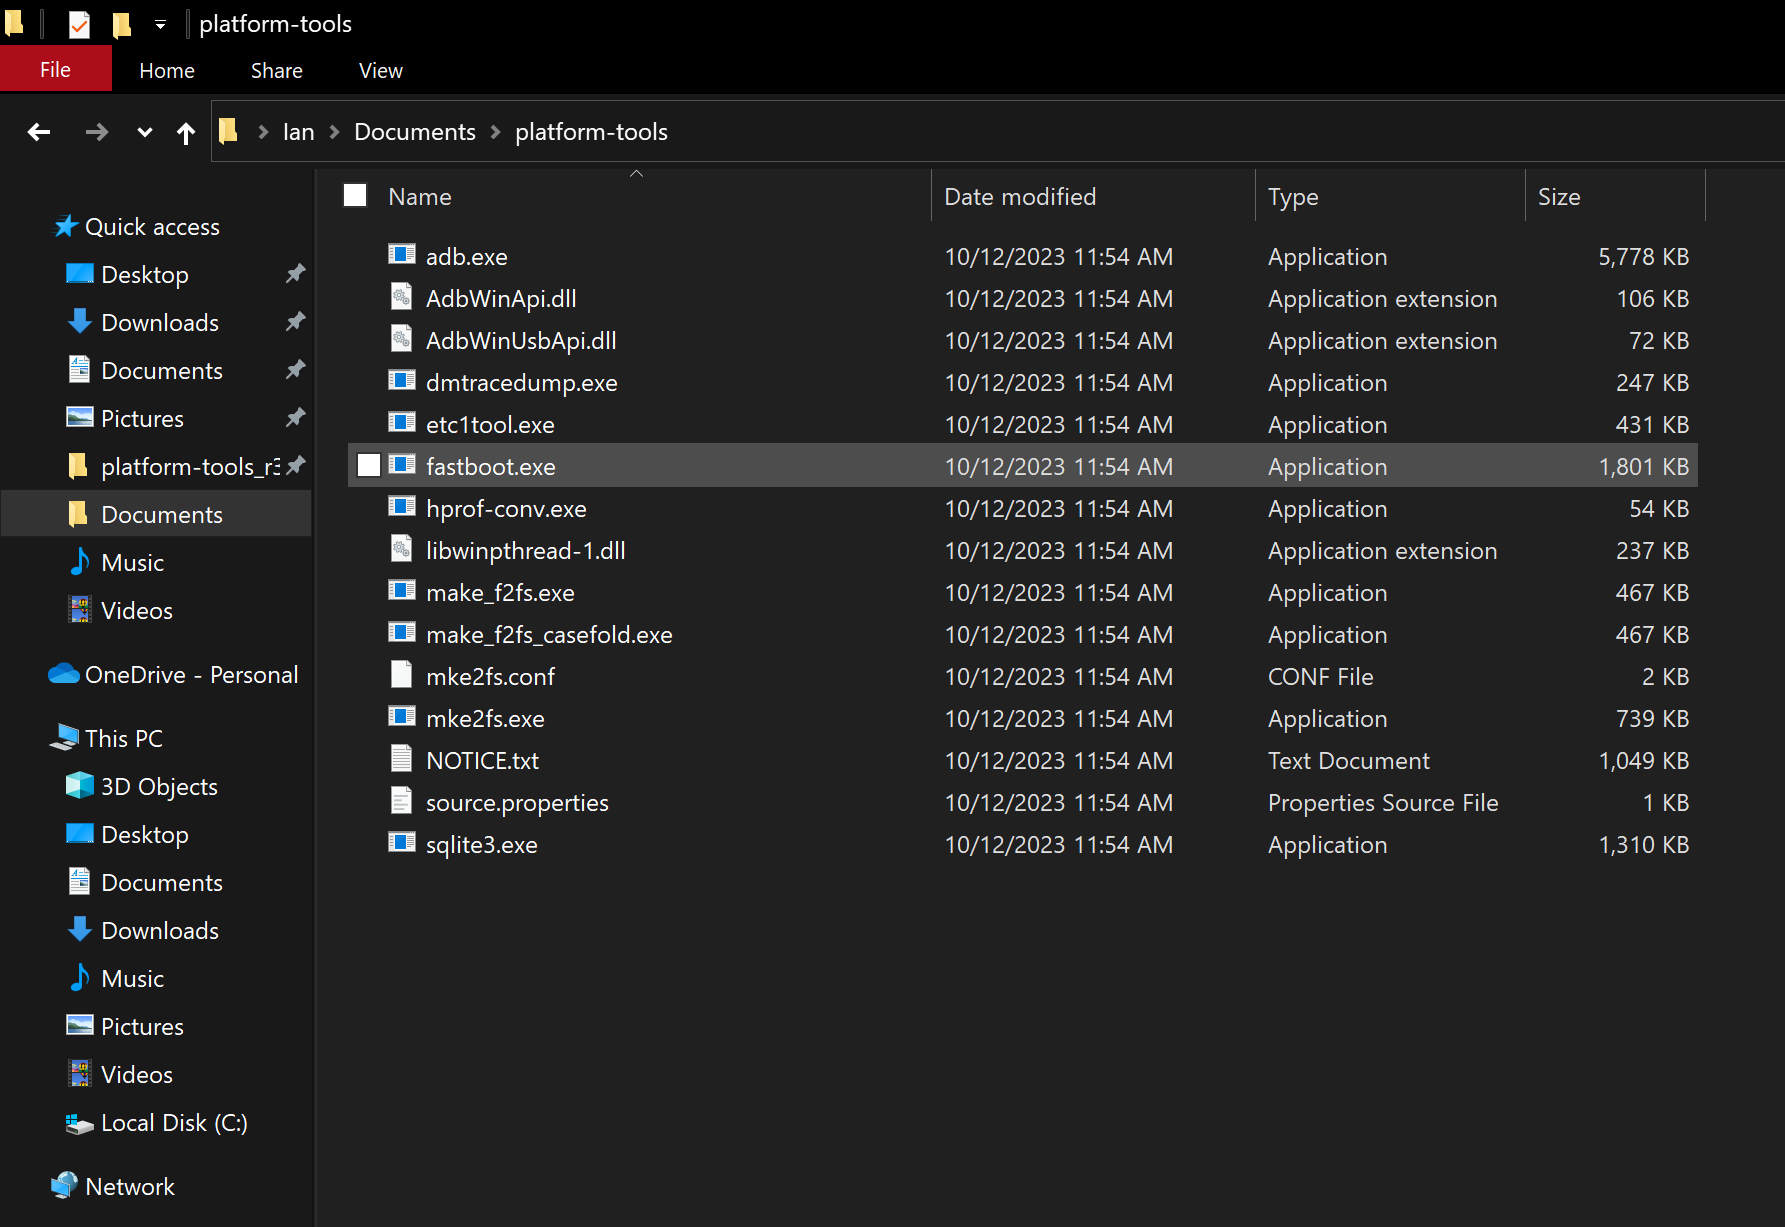
\includegraphics{PlatformTools}

\subsection{Enable USB Debugging and OEM Unlocking}
The second step to unlocking the bootloader is enabling USB debugging. This is a setting that can be enabled on an Android device in order to move files between the device 
and a computer. More specifically, enabling it allows the device to be recognized by the computer in adb mode. This makes it possible to boot the device in Fastboot mode. 
Additionally, there is another setting that must be enabled in order to further progress in rooting the device. This setting is known as OEM Unlocking. It is 
responsible for allowing the bootloader to be unlocked. In other words, it allows rooting to be possible on the device. Enabling this setting in particular is an integral
part of being able to root the device. Usually, the user would need to go into "developer options" in their settings in order to find this setting. Since this process 
doesn't change between devices, the steps to finding this setting are as follows: 

\begin{itemize}

\item Go to settings
\item Tap About Device
\item Locate the Build Number and tap it 7 times
\item Return to the main Settings screen
\item Go to System
\item Tap Developer Options

\end{itemize}

It is within "Developer Options" that the aforementioned settings can be found.

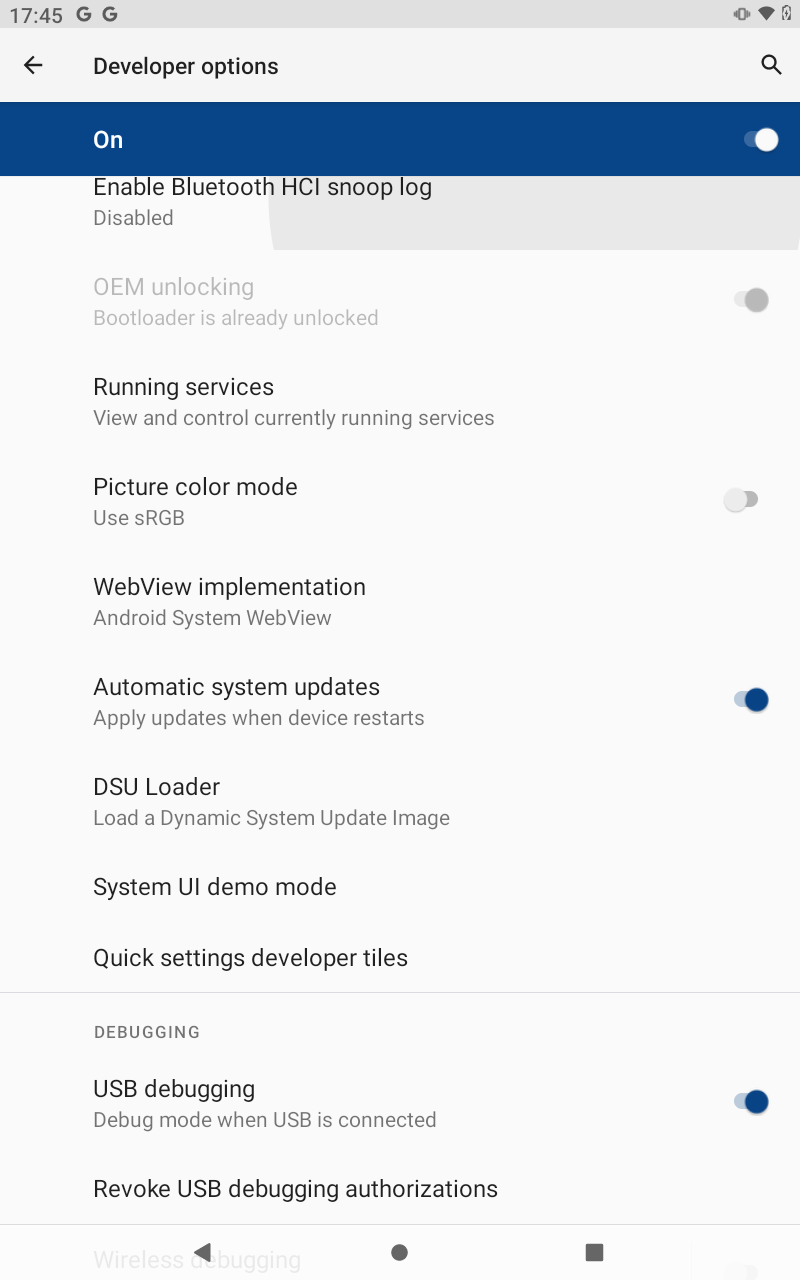
\includegraphics{DeveloperOptions}

\subsection{Boot Device to Fastboot Mode}
The third step to unlocking the bootloader is booting into Fastboot Mode. In this step, the device will have to be connected to a computer. It is necessary to 
open folder where the Android SDK Platform Tools were downloaded through the command line. Then, in order to boot the device into Fastboot Mode, type the command
"adb reboot bootloader". At this point, the device should be in Fastboot Mode. This can be verified by typing the command "fastboot devices" in the command line.
Again, Fastboot Mode allows to a Unix shell that gives the developer the ability to communicate with the device on a very low level.

\subsection{Unlock Bootloader via Fastboot Command}
This is pretty much the final step to unlocking the bootloader. In this step, only one command needs to be run in order to unlock the bootloader and root the device. 
Type the command "fastboot flashing unlock" into the command line. This command should prompt a confirmation screen to appear on the Android device. 
Once the operation is confirmed, the device should reboot automatically. If not, then type "fastboot reboot".

\section{Flash the TWRP Custom Recovery}
In order to load the device with a new operating system is to get a custom recovery. This can be done fairly simply by going to the XDA Developers forum. 
Once there, search for the tablet device in question. XDA is a great resource for everything related to rooting, modding, and custom ROMs. It is here that 
the instructions for how to get a custom recovery for the specified device will be found. Once found, download it and boot it into TWRP application. Again, 
this process is done in order to have a copy of the firmware on the device with root access. Once the custom recovery is flashed onto the device, the device should 
then be rooted. The device should be rebooted after this process.


\section{Installing Linux}
Once the device is rooted, installing Linux is a very straightforward process actually. The steps are as follows:

\begin{enumerate}

\item Connect to wifi

\item Install BusyBox

\item Install Linux Deploy

\item Open BusyBox and tap Start (this ensures that root permissions are enabled)

\item Tap Settings

\item Choose a Linux Distribution

\item Check the Enable box under GUI to view a Linux desktop

\item Open Graphics and select VNC

\item Choose the Desktop environment you want under GUI settings

\item Find the User name and User password fields and edit them 

\item Exit the menu and tap the three dots in the upper-right corner

\item Select Install, then OK

\end{enumerate}

Once those steps are completed, Linux should be installed onto the device. The desktop environment can be viewed by installing VNC Viewer which 
can be found on the Play Store. Press the start button in Linux Deploy to run Linux and then open VNC Viewer. Connect to localhost:5900 to view 
the Linux desktop.

And just like that, Linux is installed onto the tablet. That was a very simple process wasn't it? Or perhaps...maybe not...

\section{Pitfalls to trying to load another operating system}
The process of installing linux onto a tablet as described above may seem straightfoward and fairly feasible, however there are many places where this 
process fails. Many of the failures come with actually trying to root the device. One such example is finding the appropriate firmware for the tablet in use. 
Some brands of tablets aren't popular enough for their firmware to be posted for people to download. That being the case, it would be impossible to root 
the device in this scenario. This issue was the very one encountered when researching this topic. As such, the team was indeed not able to successfully root the 
tablet in order to install a Linux environment onto the device. Small encounters with issues like this are not uncommon when dealing with trying to root an 
Android device. It should be said that one should first do major research on rooting compatability before purchasing a device that they wish to root.
